\begin{frame}
\frametitle{NEXT-HD based in SiPMs}

\begin{columns}
\column{0.45\textwidth}

\blt\ An upgrade of the NEXT technology to the ton scale, based in replacing PMTs with SiPMs was proposed in 2017. The proposed detector was symmetric, with two identical sensor planes behind the transparent anodes. The sensor planes alternated large SiPMs or energy measurements, with small SiPMs for tracking measurements. 

 \column{0.45\textwidth}
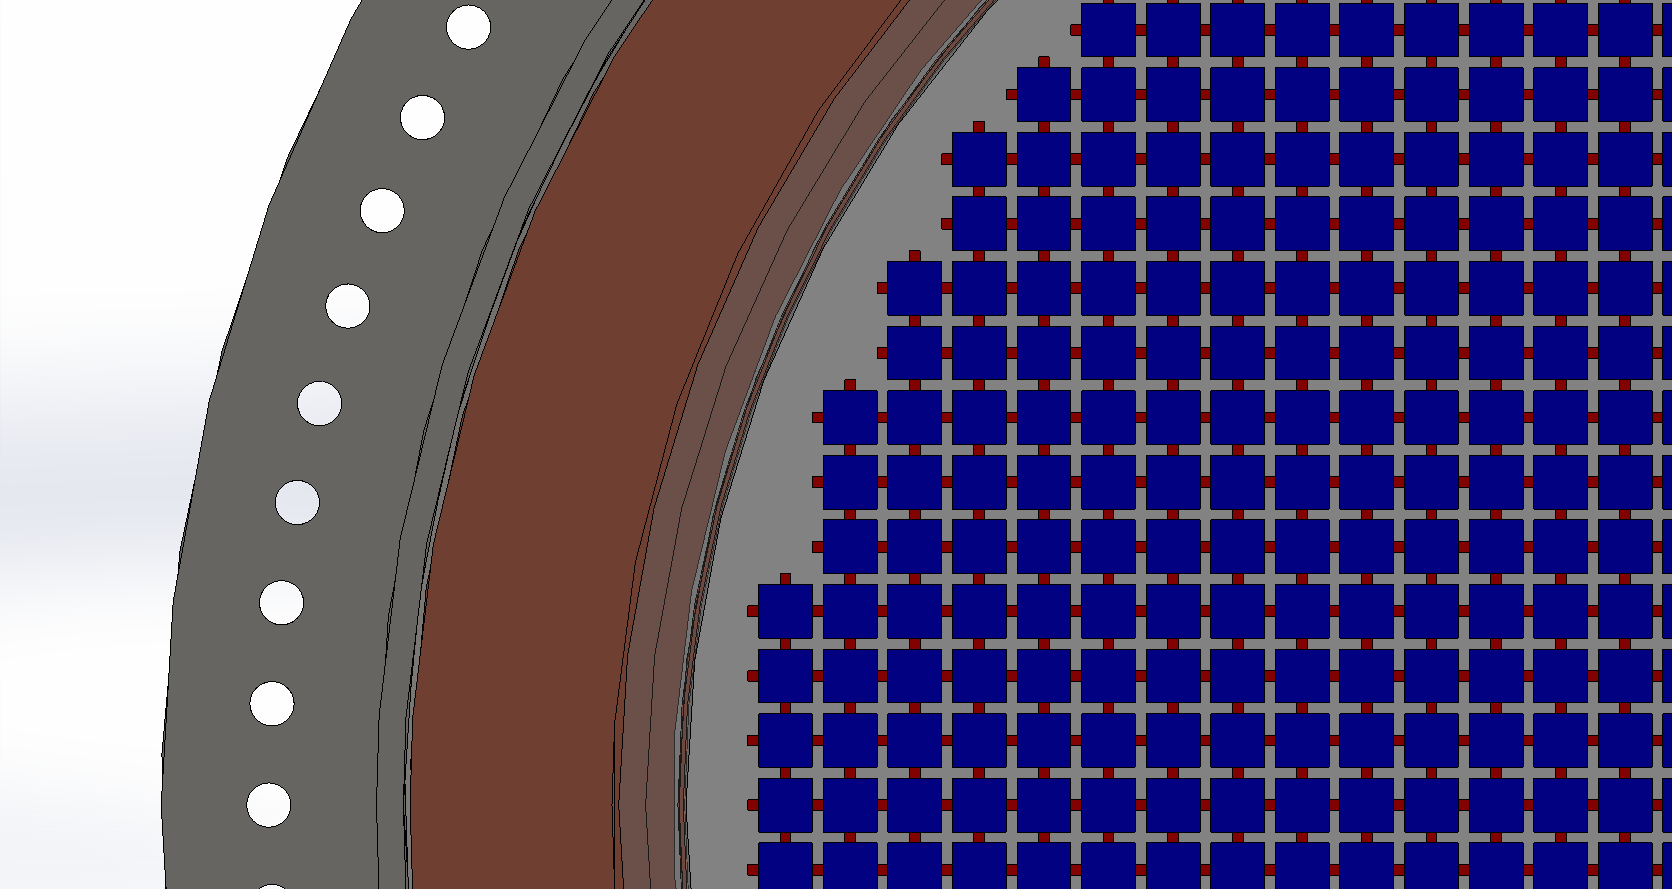
\includegraphics[scale=0.13]{img/n2-sector.png}

\end{columns}

\vspace{1cm}
{\fontsize{6pt}{7.2}\selectfont \bf Status of NEXT and prospects for a future Next Array apparatUS with Improved CApAbilities (NAUSICAA), J.J.  Gomez-Cadenas, PoS NEUTEL2017 (2018) 032.}
\end{frame}

\begin{frame}
\frametitle{NEXT-HD based in SiPMs: principle of operation}

\blt\ The small SiPMs (called tracking SiPMs or tSiPM) in each anode would perform the tracking function in the same way that currently done in \New\ and \Next.

\blt\ The large SiPMs (called energy SiPMs or eSiPM) in the opposite anode would perform the energy function, replacing the PMTs in \New\ and \Next.

\blt\ The eSiPMs of both planes would measure the primary scintillation needed for \tz.

\blt\ It was clear since the beginning that cool gas was necessary (FM, LA) to reduce DCR to manageable levels. 
\end{frame}

\begin{frame}
\frametitle{NEXT-HD based in SiPMs: size of SiPMs}

\blt\ The size of the tSiPMs can be chosen to be $\sim$\SI{1 x 1}{mm^2}, like  in \New\ and \Next.

\blt\ The eSiPMs must be chosen, a priory, as large as possible, to reduce the number of electronic channels. Choosing the eSiPMs size as \SI{10 x 10}{mm^2} results in \num{883572} channels (for a $\sim$ 90\% coverage). 

\blt\ Smaller SiPMs result in a very large number of channels (e.g, almost 3 M channels for \SI{3 x 3}{mm^2}). Reducing coverage results in reduced detection efficiency. 

\blt\ It was clear since the beginning that cool gas was necessary (FM, LA) to reduce DCR to manageable levels. 
\end{frame}

\begin{frame}
\frametitle{NEXT-HD based in SiPMs: \sone\ detection efficiency}

\blt\ The geometrical efficiency for the symmetric version of HD with SiPMs was computed by JMV to be 31.4 \%. Assuming a 40\% PDE for the SiPMs, the detection efficiency is 12.4 \%. 

\blt\ The number of scintillation photons produced by krypton deposits (assuming 
$W_s = 39.20$eV) is \num{1.06e+03}. Multiplying by the detection efficiency, one finds a total of \num{1.31e+02} detected photons from krypton. This implies an average
of \num{1.49e-04} photoelectrons per SiPM, a very small number. 

\blt\ The number of scintillation photons produced at \Qbb\ is \num{1.12e+05}. Multiplying by the detection efficiency, one finds a total of \num{7.78e+03} detected photons from krypton. This implies an average
of \num{8.80e-03} photoelectrons per SiPM, still a small number. 

\end{frame}

\begin{frame}
\frametitle{NEXT-HD based in SiPMs:  SiPM response}

\begin{columns}
\column{0.45\textwidth}

\blt\ Large SiPMs have large capacitance. A SiPM of \SI{10 x 10}{mm^2} has a capacitance of \SI{10}{ns}. As a consequence, the output waveform when connected to a readout will have a very long decay time, of the order of \SI{5}{\micro\second}.

\blt\ This implies that the output of the fast \sone\ signal will be a waveform which needs to be integrated up to \SI{5}{\micro\second}

 \column{0.45\textwidth}
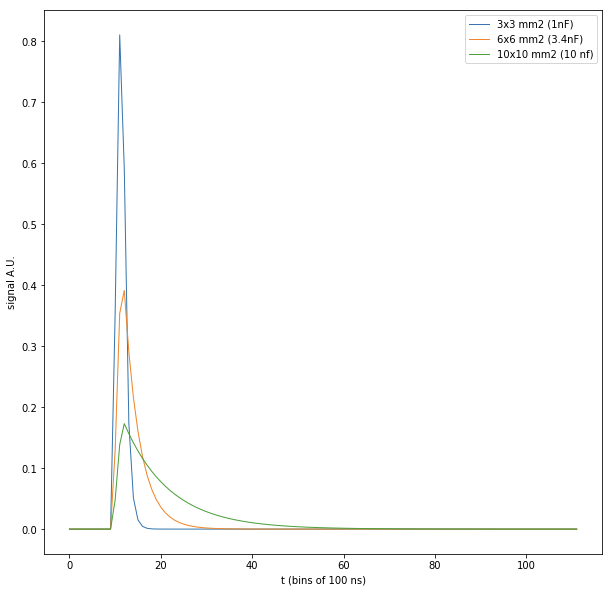
\includegraphics[scale=0.23]{img/sipmResponse.png}

\end{columns}
\end{frame}

\begin{frame}
\frametitle{NEXT-HD based in SiPMs:  DCR}

\begin{columns}
\column{0.45\textwidth}

\blt\ The dark current rate (DCR) of SiPMs is of the order of \SI{100}{\kilo\hertz\per\mm^2}, but decreases rapidly with temperature. 

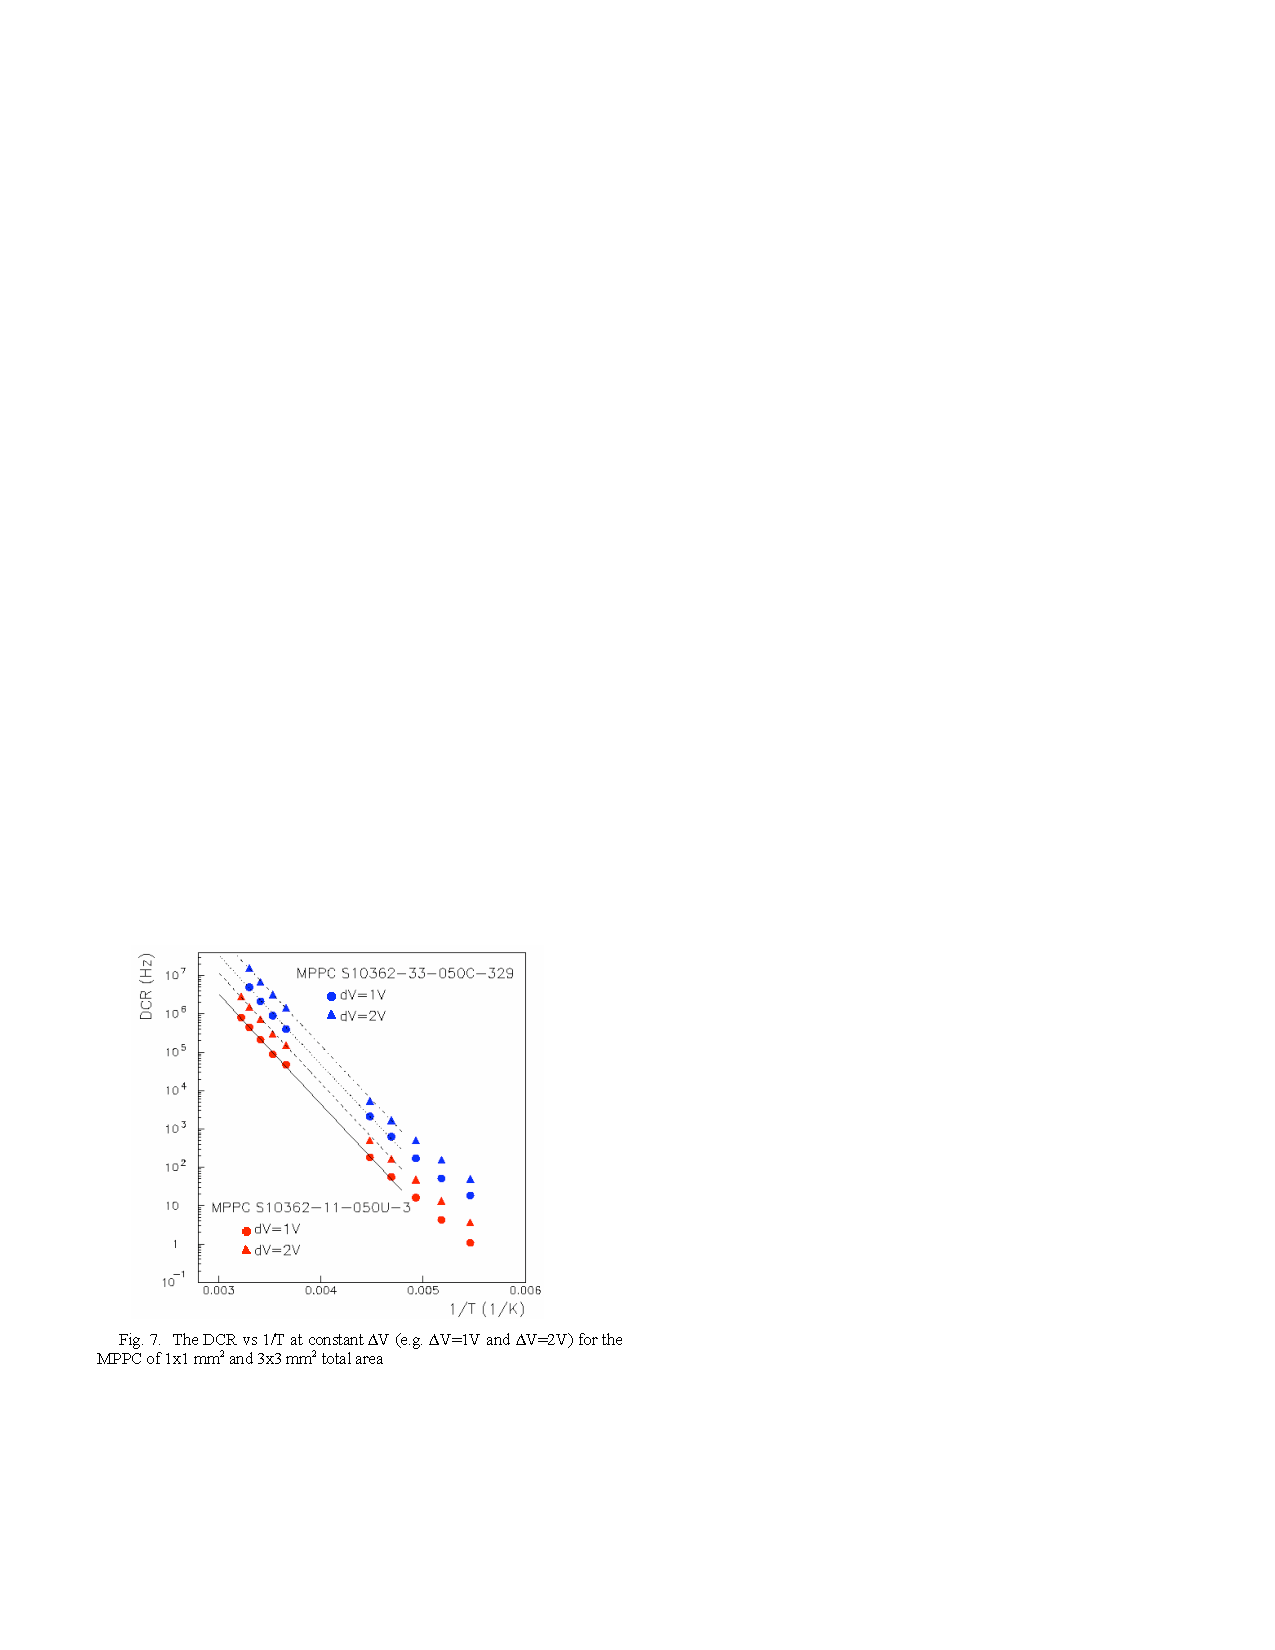
\includegraphics[scale=0.63]{img/dcR_T.pdf}

 \column{0.45\textwidth}
 
 \blt\ Unfortunately the noise per SiPM of \SI{10 x 10}{mm^2} in \SI{5}{\micro\second} is always larger than the \sone\ signal expected per SiPM at \Qbb

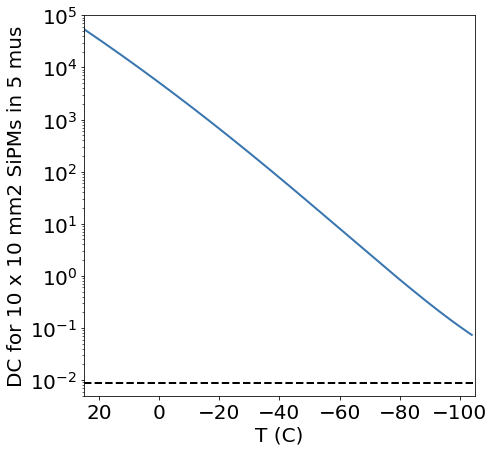
\includegraphics[scale=0.3]{img/dcr5mus.png}

\end{columns}

\blt Measuring \tz\ with a detector based in SiPMs is very difficult. 
\end{frame}


